\section{Déroulement du projet}

\subsection{Systemtap}

\subsubsection{Principe de fonctionnement}

Nous avons ainsi commencé par utiliser Systemtap, un outil d'analyse du noyau grâce à des scripts qui ne nécessitent pas de modifier le code du noyau. Systemtap utilise les KProbes, et les Kretprobes\cite{IBMRBST} pour intervenir à différents endroits dans le déroulement des fonctions du noyau pour permettre à l'utilisateur de lire certaines variables ou de logger certains appels système. Le principe de fonctionnement de Systemtap est résumé sur le schéma ci-dessous.

\begin{figure}[hb]
	\centering
	\includegraphics[scale=0.4]{kretprob.png}
	\caption{Fonctionnement tel que décrit dans la référence IBM sur Systemtap \cite{IBMRBST}}
\end{figure}

\subsubsection{Résultats obtenus}

Après s'être familiarisé avec le fonctionnement de Systemtap, nous nous sommes aperçu que les scripts utilisés pour récupérer les informations issues des appels système sont exécutés une fois l'appel système effectué. Il n'est pas possible, d'après nos recherches, de faire en sorte que les scripts puissent bloquer les appels système avant de les effectuer.

De ce fait, l'utilisation de Systemtap ne permet pas de répondre à nos besoins.

Il faut ajouter à cela que les informations recueillies à partir de Systemtap ne sont pas exploitables pour certaines d'entre-elles. Par exemple, lorsqu'un fichier est accédé (lu ou écrit), seul le numéro d'inode nous était retourné. Il n'était alors pas pertinent de récupérer le chemin complet du fichier, car cette recherche est inadaptée et inefficace : il est nécessaire de parcourir l'intégralité du système de fichiers.

Il fallait donc changer de stratégie. C'est pourquoi, nous avons, avec l'accord du responsable du projet, décidé de nous orienter vers l'utilisation des ``Linux Security Modules'' (LSM).

\subsection{Linux Security Modules}

\subsubsection{Principe de fonctionnement}

Les modules LSM sont au noyau ce que netfilter est au réseau.

Le principe de fonctionnement est simple : un module LSM est chargé dans le noyau Linux au démarrage. Il se substitue ou complète alors la procédure de contrôle d'accès. \`A chaque appel système est associé un hook que l'on peut considérer comme une fonction. Il est placé dans l'appel système entre les vérifications élémentaires (existence des fichiers, droits unix) et sa réalisation. Dès qu'un appel système est demandé, le hook est exécuté. Par défaut, il autorise l'exécution de l'appel système.

\begin{figure}[hb]
	\centering
	\includegraphics[scale=0.45]{lsm1.png}
	\caption{Architecture des hooks LSM \cite{LSMINTRO}}
\end{figure}

L'avantage de ces hooks est qu'ils offrent une très grande liberté. Cependant, il n'est possible pour le moment que de charger dans le noyau qu'un seul et unique module LSM. Or, PIGA utilise déjà un module LSM modifié, celui de SELinux.

Pour simplifier le développement, nous avons désactivé SELinux. \`A terme, il se pourrait que SELinux soit définitivement désactivé.

\begin{figure}%[hb]
	\centering
	\includegraphics[scale=0.45]{lsm2.png}
	\caption{Hook LSM permissif. Ce hook autorise la politique de sécurité à passer outre les restrictions DAC \cite{LSMINTRO}}
\end{figure}

L'avantage de ces hooks est qu'ils offrent une très grande liberté. Cependant, il n'est possible pour le moment que de chargé dans le noyau qu'un seul et unique module LSM. Or, PIGA-OS utilise déjà un module LSM : SELinux.

Pour les besoins du développement, nous avons dû désactiver SELinux, pour nous concentrer sur notre propre module, et non sur l'intégration avec le module LSM de SELinux.

\subsubsection{Implémentation}

Nous avons donc développé un module LSM qui "hook" les appels système. Par défaut, ces hooks sont "transparents" à l'exception du hook "file permission" sur lequel nous travaillons. Il est appelé à chaque ouverture (lecture, écriture, exécution) de descripteur de fichier.

Par la suite, il faudra convenir des appels systèmes sur lesquels il est intéressant d'intervenir.

Nous avons ajouté la possibilité d'activer ou non ce module lors de la compilation du noyau en suivant les conventions de nommage des options de configuration.

Ensuite, nous avons commencé à chercher les différentes informations nécessaires à contextd pour son fonctionnement, et plus particulièrement ce qui concerne le hook "file permission" :
	\begin{itemize}
		\item le PID
		\item l'execname
		\item le chemin complet du fichier
		\item ...
	\end{itemize}

Nous avons également remarqué que le hook "socket bind" permet de récupérer des informations, notamment l'adresse IP et le port de destination d'une socket, avant qu'elle ne soit créée. Son fonctionnement doit être confirmé, car il pourrait nous affranchir d'utiliser une alternative telle que ULOG et iptables.
% 	\begin{itemize}
% 		\item[-] le PID
% 		\item[-] l'execname
% 		\item[-] la structure de la socket
% 		\item[-] L'adresse de connexion
% 		\item[-] ...
% 	\end{itemize}

La principale difficulté de cette étape était de localiser dans quels fichiers ses informations sont localisées dans l'ensemble du code source du noyau Linux.

L'étape suivante consiste à envoyer les informations récupérées dans l'espace noyau à l'espace utilisateur. Nous avons envisagé plusieurs pistes, pour l'instant restées infructueuses.

\newpage

\subsection{Idées abandonnées}

\subsubsection{Socket Unix}

Tout d'abord, nous avons essayé de créer une socket Unix pour communiquer avec l'espace utilisateur. Cependant, les sockets NETLINK ne garantissent pas que les informations soient correctement envoyées. Il devient alors difficile de maîtriser le comportement du hook : il n'y a donc aucune garantie quant à la poursuite ou non de l'appel système.

\subsubsection{Proc fs}

Cette solution consiste à créer un ou plusieurs devices dans /proc. Le noyau écrirait dans l'un et lirait les réponses dans l'autre. Or cette solution ne permet pas de s'assurer facilement que seul un processus écrit et lit et donc d'authentifier les échanges entre le noyau et le démon. De plus il est nécessaire de parser les informations transmises par un device.

\subsection{Interface et appels système}

Nous avons envisagé de créer trois nouveaux appels systèmes pour répondre au besoins de communications entre le noyau et contextd. Un appel système nous permet de renseigner et de transmettre une structure avec toutes les informations nécessaires à contextd. Cela nous évite ansi de parser du texte et facilite le processus d'authentification du démon qui correspond alors à un simple appel système lui aussi. La procédure d'authentification est une procédure séparée.

\begin{figure}[hb]
	\centering
	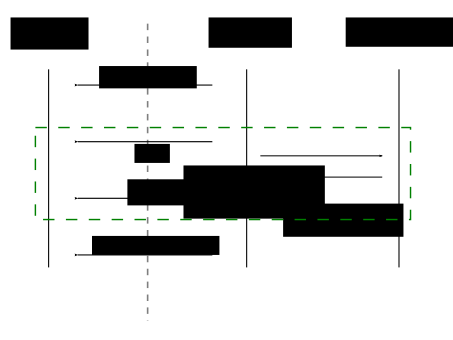
\includegraphics{global.pdf}
	\caption{Communication entre le noyau, le démon et contextd}
\end{figure}
%
Il faut donc s'assurer que le démon se désauthentifie si le processus est terminé. \`A terme, ce comportement ne sera pas accepté.

Nous utilisons des mutex pour contrôler les échanges d'informations entre le noyau et le démon et assurer le traitement de chacun des appels système.

\begin{figure}[hb]
	\centering
	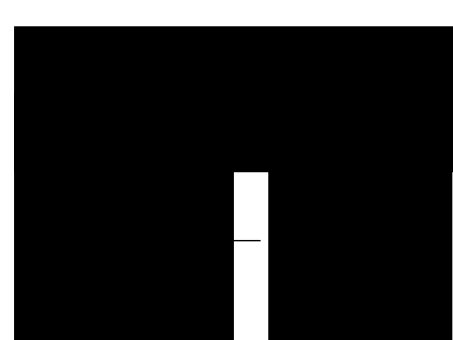
\includegraphics{syscall_sync.pdf}
	\caption{Communication entre les hooks LSM et les appels système}
\end{figure}